Regarding the ultimate goal of deriving policy recommendations (Obj.~4 in \sref{s:intro:aim-objectives}), no particular welfare (economic) assessment tool was used. The recommendations are general guidelines, not specific numbers on, for example, environmental taxes, thus the decision was made to avoid using a formal economic assessment method. Instead, the policies were \emph{informed} by the transition studies perspective \parencite{kemp2007_Transitionmanagementas}, which integrates the results of the backcasting process (the transition pathway) and the analysis of the feedback structures in the current mobility system through the use of CLDs.

The integration of the rest of the results through a transitions perspective was done by analysing those same insights through a different \emph{discourse}. The formal method used for rising the CLD and backcasting outcomes to the same discursive level is the so called \emph{\gls{MLP}}. This analytical framework defines three levels that characterise a socio-technical system \parencite{geels2001_Technologicaltransitionsas}. These levels are associated with micro, meso and macro perspectives, as portrayed in \fref{f:mlp-methods} \parencite{rotmans2001_Moreevolutionthan}:
\begin{enumeratealpha}
\item The socio-technical \emph{niche} level, at the most microscopic level of the system, is the location where radical innovation occurs. Several processes occur within the niches: the articulation of expectations (visions), the construction of stakeholder networks and learning on different dimensions (organisational, policy, technological, etc.) \parencite{geels2012_MultiLevelPerspective}.
\item The socio-technical \emph{regime} level is situated at the mesoscopic level. It is the virtual space formed by all the actors within a socio-technical system, their shared practices, rules and cultures. Infrastructure supporting the socio-technical system, as well as regulation, and technology belong to the regime level too. In the case of regimes, innovation is not radical. Instead, it is incremental and rather slow, following a pattern of ``dynamic stability''. Resilience is, thus, a key characteristic of regimes \parencite{geels2012_MultiLevelPerspective}.
\item The socio-technical landscape, at the macroscopic level, is the context in which both regimes and niches are embedded. Ideologies, culture, value hierarchies, beliefs, macroeconomic trends, the media, governance systems, etc. belong to this level. The landscape shapes, through pressures and support relations, the regimes and the niches. A characteristic of this level is the slow changes it suffers: regimes come and go, even more so niches, but it can take several decades or even centuries for change in the landscape to become apparent \parencite{rotmans2001_Moreevolutionthan,kemp2007_Transitionmanagementas,geels2012_MultiLevelPerspective}.
\end{enumeratealpha}

\begin{figure}
\centering
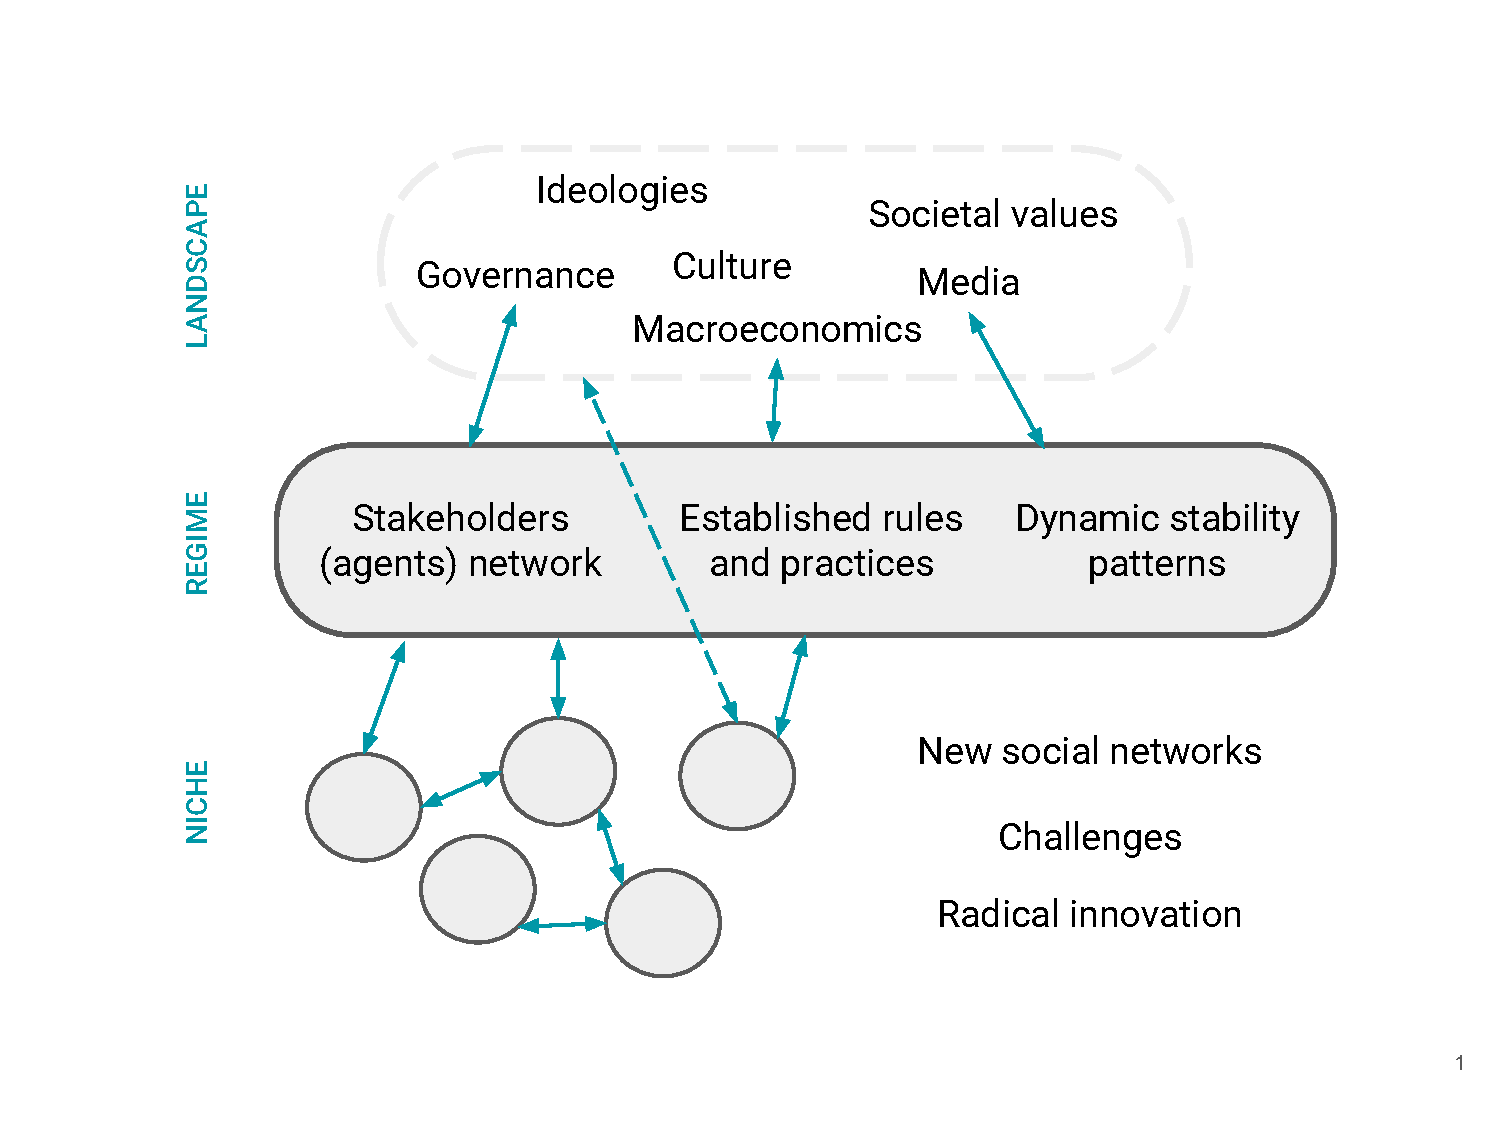
\includegraphics[width=0.8\linewidth,trim=0 2cm 0 2cm,clip]{figures/mlp.pdf}
\caption[The Multi-Level Perspective]{The Multi-Level Perspective analytical framework, with the macro, meso and micro levels visible.}
\label{f:mlp-methods}
\end{figure}

The MLP allows for a multi-dimensional analysis of mobility, because it deals with more than just technologies (or any other aspect of the system: economics, environmental impacts, regulation, etc.). This is ideal to overcome the limitations in scope of traditional transport research identified in the \nameref{s:intro:state-of-art} section. The MLP also addresses structural change by analysing how socio-technical innovations fight for dominance against established regimes. Structural change is an important element in transitions that previous mobility research (or policy) tends to obviate. The MLP also stresses the importance of the patterns of co-evolution between the landscape and regimes and niches. In particular, the MLP (and transitions studies in general) addresses the dynamics of stability and change of regimes and niches \parencite{geels2011_multilevelperspective}. This specific feature of the MLP serves very well the aim of the thesis of understanding why mobility presents policy resistance and what can be done to tackle it.

Finally, the way in which the MLP is used in the thesis is as follows: the backcasted changes (Objs.~1,2) that conform the transition pathway are described in the terms of the MLP. The feedback mechanisms that cause policy resistance in today's mobility system (Obj.~3) are then incorporated to the description and also translated into the language of the MLP. Thus, the narration of the transition path contains: (1) normative elements on a broad range of dimensions, stemming from the backcast and (2) a dynamic analysis of the forces that can hinder the transition nowadays. This MLP-inspired analysis is finally used to design a set of policy recommendations that focuses both on the long term goals and on breaking the resilience of the current mobility system that poses an obstacle to its own radical transformation (Obj.~4).